\documentclass[12pt, a4paper, oneside]{ctexart}
\usepackage{amsmath, amsthm, amssymb, graphicx,fancyhdr,geometry , subfigure}
\usepackage[bookmarks=true, colorlinks, citecolor=blue, linkcolor=black]{hyperref}
\geometry{a4paper,scale=0.75}
\pagestyle{fancy}
\fancyhf{} 
\fancyhead[L]{千斤顶成套设计说明书}
\fancyhead[C]{} % Center header - document title
\fancyhead[R]{王德茂} % Right header - page number
\fancyfoot[C]{\thepage}
\begin{document}

\ctexset{
  abstractname = {}
  
}

\title{\textbf{千斤顶成套设计说明书}}
\author{王德茂}
\date{\today}
\maketitle

\begin{abstract}
  \begin{center}
    \textbf{摘要}
\end{center}
  
  
  本文全面阐述了千斤顶成套设备的设计流程和规格。首先明确了设计目的和性能标准,涉及承重、起始位置、升降高度和重量上限。随后,探讨了成本和特殊需求,着重于成本控制和电动功能,加入了电动系统。最终,提供了装配和零件图纸,以便于制造和组装。
    
    \noindent{\textbf{关键词:}千斤顶、设计、机械}
\end{abstract}

\begin{abstract}
  \begin{center}
    \textbf{Abstract}
\end{center}

  This article comprehensively explains the design process and specifications of jack complete equipment. First, the design purpose and performance standards were clarified, including load-bearing, starting position, lifting height and upper weight limit. Subsequently, costs and special needs were discussed, focusing on cost control and electric features, and electric systems were added. Finally, comprehensive assembly and parts drawings are provided to facilitate fabrication and assembly.
    
    \noindent{\textbf{Keywords:} Jack, design, machinery}
\end{abstract}
\newpage
\section{设计要求表}
本设计旨在开发一款高性能、低成本、电动化的千斤顶成套设备,以满足不同场合下的重型举升需求。具体要求如下:
\begin{itemize}
  \item \textbf{功能要求}:千斤顶应具备承载能力强、初始位置低、顶升高度可调、重量轻便等特点。
    \begin{itemize}
    \item \textbf{承载能力}:千斤顶能够承受的最大重量,本设计要求千斤顶能够承载2吨(2000kg)的重物。
    \item \textbf{初始位置}:千斤顶的最低工作位置,应确保其能够在地面水平位置进行操作。
    \item \textbf{顶升高度}:千斤顶能够达到的最高工作位置,可根据需要调整其顶升高度。
    \item \textbf{重量限制}:千斤顶的整体重量不应超过20kg,便于移动和安装。
    \end{itemize}
  \item \textbf{经济要求}:考虑到成本效益,千斤顶的设计应力求降低生产成本,同时确保设备的性能稳定可靠。
    \begin{itemize}
    \item \textbf{成本控制}:千斤顶的总成本不应超过2000元人民币。
    \end{itemize}
  \item \textbf{特殊需求}:由于某些应用场景的特殊需求,千斤顶需具备电动操作功能,以便于远程控制和提高效率。
\end{itemize}

\begin{table}[htbp]
\centering
\begin{tabular}{|c|c|}
  \hline
\textbf{项目} & \textbf{要求} \\
\hline
功能 & 1. 承重:2000kg\\
     & 2. 初始位:地面\\
     & 3. 顶升位:最高1m\\
     & 4. 重量:$\leq20$kg \\
     \hline
经济 & 成本:$\leq2000$元 \\
\hline
特殊需求 & 电动 \\
\hline
\end{tabular}
\caption{设计要求简述}
\end{table}

\section{初步思考原理方案}
在设计千斤顶的初步思考原理方案时,我们分析了各种可能的传动方式和驱动机制,以找到最适合本设计要求的方案。在比较了多种传动方式如液压、气动、机械齿条和螺旋传动后,我们最终选择了螺旋千斤顶作为基础设计,并在其上增加了电动驱动系统。

我们选择备选1,因为我们想实现电动设置,而备选2在工作时要想实现电动,没有合适的思路。

考虑到,一般要用到电动的设备,可能是在一些专业的维修厂之类,所以工作时应该可以有比较大的工作空间,并且不用太担心重量。

\begin{figure}[htbp]
  \centering
  \subfigure[备选1]{
  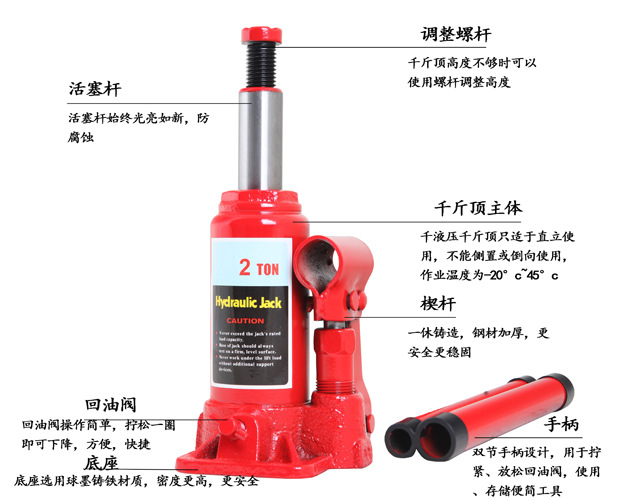
\includegraphics[scale=0.25]{image_1.png} \label{1}
  }
  \quad
  \subfigure[备选2]{
  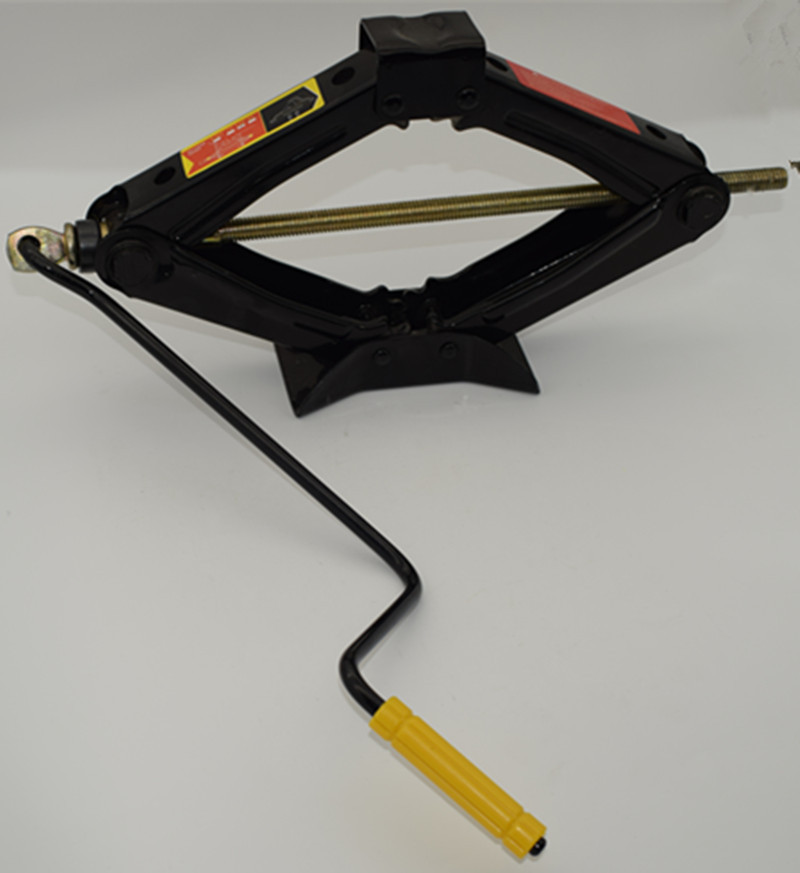
\includegraphics[scale=0.15]{image.png} \label{2} 
  }
  
  \caption{设计方案选择}


\end{figure}
\begin{itemize}
  \item \textbf{螺旋传动}:通过螺旋副的啮合,可以将旋转运动转化为线性运动,实现千斤顶的升降功能。这种传动方式效率高、结构简单。
  \item \textbf{电动驱动}:为了提高效率和便利性,我们在螺旋千斤顶的基础上增加了电动驱动系统。电动机可以通过电力驱动千斤顶,实现远程控制和快速响应。
\end{itemize}

\section{设计计算说明}
在设计过程中,我们对关键部件进行了详细的计算和分析,以确保整个系统的安全和稳定性。

\begin{itemize}
  \item \textbf{结构强度计算}:
    \begin{itemize}
    \item \textbf{材料选择}:Q235钢,因其具有良好的强度和耐腐蚀性能。
    \item \textbf{截面尺寸}:$b \times h$,根据载荷和应力分布进行优化设计。
    \item \textbf{应力计算}:根据材料的许用应力和实际工作条件,计算出各部分的应力状态。
    \item \textbf{安全系数}:$n = 1.5$,以确保结构在服役期间的安全可靠性。
    \end{itemize}
\end{itemize}

\section{设计校核说明}
在校核过程中,我们重点关注了螺旋副、电动机驱动系统和整体结构的强度和耐久性。

\begin{itemize}
  \item \textbf{螺旋副校核}:
    \begin{itemize}
    \item \textbf{螺纹磨损寿命}:通过计算螺纹副的磨损寿命,确保其在规定使用寿命内不会出现严重损坏。
    \item \textbf{螺纹副强度校核}:检查螺纹副在不同工况下的强度是否满足设计要求。
    \end{itemize}
  \item \textbf{电动机驱动校核}:
    \begin{itemize}
        \item \textbf{电机温升校核}:确保电机在运行过程中的温度不超过其额定温度,以免影响其性能和寿命。
        \item \textbf{电机负载校核}:验证电机在满载情况下的输出能力和效率。
        \end{itemize}
      \item \textbf{结构强度校核}:
        \begin{itemize}
        \item \textbf{截面尺寸校核}:检查截面尺寸是否合理,能否有效抵抗外力作用。
        \item \textbf{材料强度校核}:确认所选材料是否能满足设计要求的强度和耐久性。
        \end{itemize}
    \end{itemize}
    
    \section{装配图和零件图}
    为了方便生产和组装,我们提供了千斤顶相关图和主要零件图,包括电机、支撑结构和底座等。这些图纸详细展示了各个部件的形状、尺寸和相互关系,确保了生产的准确性和一致性。
    
    \begin{figure}[htbp]
        \centering
        \subfigure[三维视图]{
        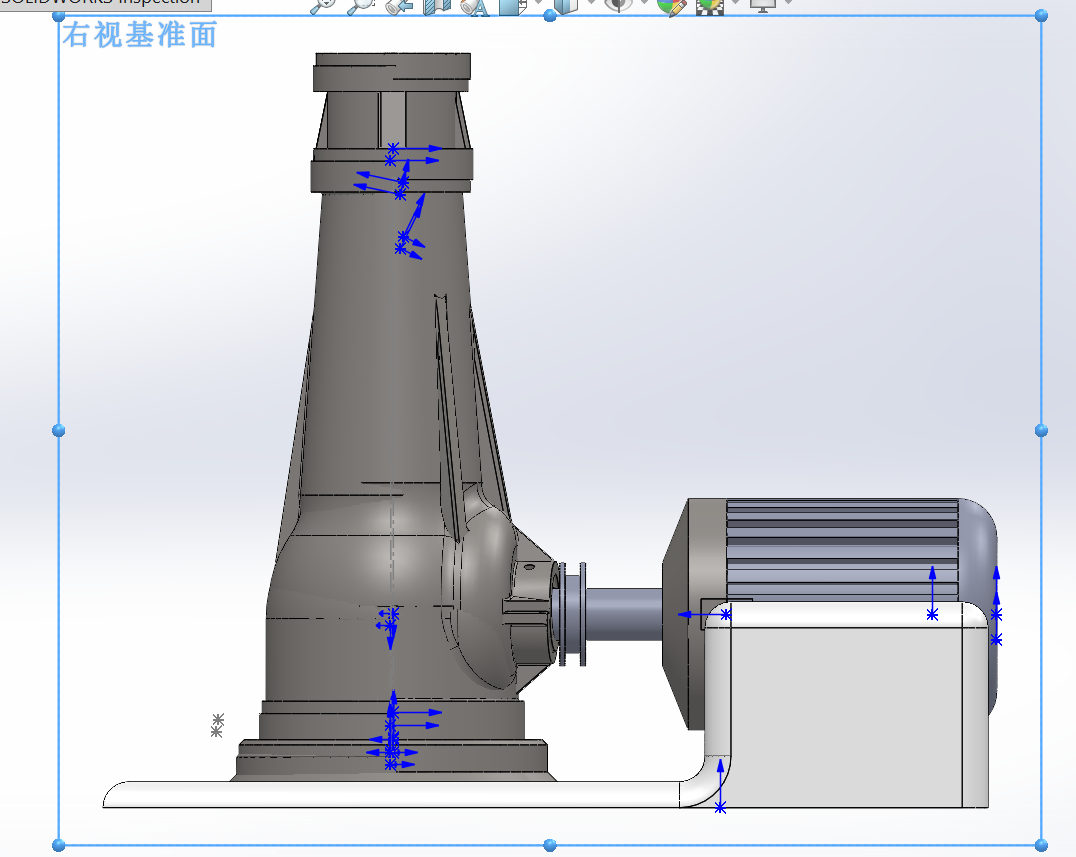
\includegraphics[scale=0.25]{image1.png} \label{1}
        }
        \quad
        \subfigure[二维图纸]{
        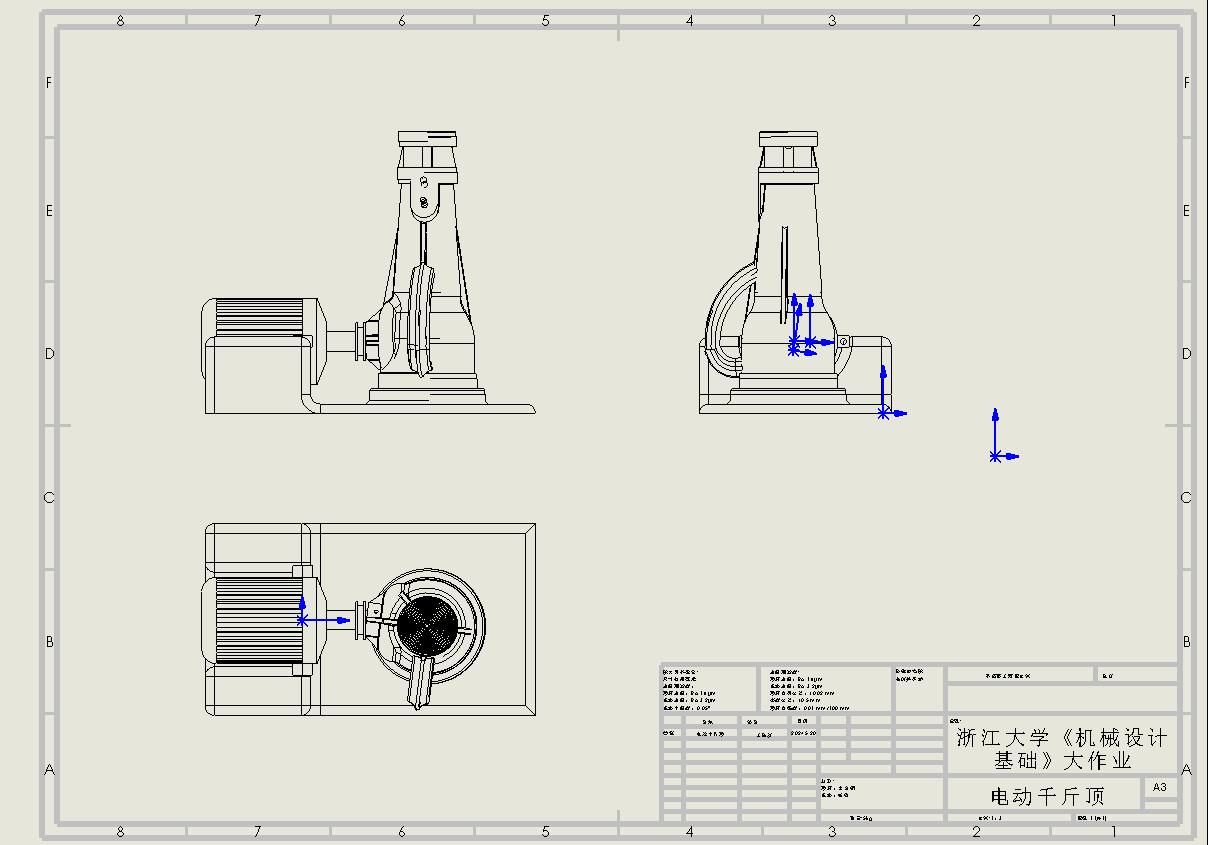
\includegraphics[scale=0.25]{imag2.png} \label{2} 
        }
        
        \caption{设计图纸}
    \end{figure}
        
\end{document}